% Options for packages loaded elsewhere
\PassOptionsToPackage{unicode}{hyperref}
\PassOptionsToPackage{hyphens}{url}
\PassOptionsToPackage{dvipsnames,svgnames,x11names}{xcolor}
%
\documentclass[
  letterpaper,
  DIV=11,
  numbers=noendperiod]{scrartcl}

\usepackage{amsmath,amssymb}
\usepackage{lmodern}
\usepackage{iftex}
\ifPDFTeX
  \usepackage[T1]{fontenc}
  \usepackage[utf8]{inputenc}
  \usepackage{textcomp} % provide euro and other symbols
\else % if luatex or xetex
  \usepackage{unicode-math}
  \defaultfontfeatures{Scale=MatchLowercase}
  \defaultfontfeatures[\rmfamily]{Ligatures=TeX,Scale=1}
\fi
% Use upquote if available, for straight quotes in verbatim environments
\IfFileExists{upquote.sty}{\usepackage{upquote}}{}
\IfFileExists{microtype.sty}{% use microtype if available
  \usepackage[]{microtype}
  \UseMicrotypeSet[protrusion]{basicmath} % disable protrusion for tt fonts
}{}
\makeatletter
\@ifundefined{KOMAClassName}{% if non-KOMA class
  \IfFileExists{parskip.sty}{%
    \usepackage{parskip}
  }{% else
    \setlength{\parindent}{0pt}
    \setlength{\parskip}{6pt plus 2pt minus 1pt}}
}{% if KOMA class
  \KOMAoptions{parskip=half}}
\makeatother
\usepackage{xcolor}
\setlength{\emergencystretch}{3em} % prevent overfull lines
\setcounter{secnumdepth}{-\maxdimen} % remove section numbering
% Make \paragraph and \subparagraph free-standing
\ifx\paragraph\undefined\else
  \let\oldparagraph\paragraph
  \renewcommand{\paragraph}[1]{\oldparagraph{#1}\mbox{}}
\fi
\ifx\subparagraph\undefined\else
  \let\oldsubparagraph\subparagraph
  \renewcommand{\subparagraph}[1]{\oldsubparagraph{#1}\mbox{}}
\fi

\usepackage{color}
\usepackage{fancyvrb}
\newcommand{\VerbBar}{|}
\newcommand{\VERB}{\Verb[commandchars=\\\{\}]}
\DefineVerbatimEnvironment{Highlighting}{Verbatim}{commandchars=\\\{\}}
% Add ',fontsize=\small' for more characters per line
\usepackage{framed}
\definecolor{shadecolor}{RGB}{241,243,245}
\newenvironment{Shaded}{\begin{snugshade}}{\end{snugshade}}
\newcommand{\AlertTok}[1]{\textcolor[rgb]{0.68,0.00,0.00}{#1}}
\newcommand{\AnnotationTok}[1]{\textcolor[rgb]{0.37,0.37,0.37}{#1}}
\newcommand{\AttributeTok}[1]{\textcolor[rgb]{0.40,0.45,0.13}{#1}}
\newcommand{\BaseNTok}[1]{\textcolor[rgb]{0.68,0.00,0.00}{#1}}
\newcommand{\BuiltInTok}[1]{\textcolor[rgb]{0.00,0.23,0.31}{#1}}
\newcommand{\CharTok}[1]{\textcolor[rgb]{0.13,0.47,0.30}{#1}}
\newcommand{\CommentTok}[1]{\textcolor[rgb]{0.37,0.37,0.37}{#1}}
\newcommand{\CommentVarTok}[1]{\textcolor[rgb]{0.37,0.37,0.37}{\textit{#1}}}
\newcommand{\ConstantTok}[1]{\textcolor[rgb]{0.56,0.35,0.01}{#1}}
\newcommand{\ControlFlowTok}[1]{\textcolor[rgb]{0.00,0.23,0.31}{#1}}
\newcommand{\DataTypeTok}[1]{\textcolor[rgb]{0.68,0.00,0.00}{#1}}
\newcommand{\DecValTok}[1]{\textcolor[rgb]{0.68,0.00,0.00}{#1}}
\newcommand{\DocumentationTok}[1]{\textcolor[rgb]{0.37,0.37,0.37}{\textit{#1}}}
\newcommand{\ErrorTok}[1]{\textcolor[rgb]{0.68,0.00,0.00}{#1}}
\newcommand{\ExtensionTok}[1]{\textcolor[rgb]{0.00,0.23,0.31}{#1}}
\newcommand{\FloatTok}[1]{\textcolor[rgb]{0.68,0.00,0.00}{#1}}
\newcommand{\FunctionTok}[1]{\textcolor[rgb]{0.28,0.35,0.67}{#1}}
\newcommand{\ImportTok}[1]{\textcolor[rgb]{0.00,0.46,0.62}{#1}}
\newcommand{\InformationTok}[1]{\textcolor[rgb]{0.37,0.37,0.37}{#1}}
\newcommand{\KeywordTok}[1]{\textcolor[rgb]{0.00,0.23,0.31}{#1}}
\newcommand{\NormalTok}[1]{\textcolor[rgb]{0.00,0.23,0.31}{#1}}
\newcommand{\OperatorTok}[1]{\textcolor[rgb]{0.37,0.37,0.37}{#1}}
\newcommand{\OtherTok}[1]{\textcolor[rgb]{0.00,0.23,0.31}{#1}}
\newcommand{\PreprocessorTok}[1]{\textcolor[rgb]{0.68,0.00,0.00}{#1}}
\newcommand{\RegionMarkerTok}[1]{\textcolor[rgb]{0.00,0.23,0.31}{#1}}
\newcommand{\SpecialCharTok}[1]{\textcolor[rgb]{0.37,0.37,0.37}{#1}}
\newcommand{\SpecialStringTok}[1]{\textcolor[rgb]{0.13,0.47,0.30}{#1}}
\newcommand{\StringTok}[1]{\textcolor[rgb]{0.13,0.47,0.30}{#1}}
\newcommand{\VariableTok}[1]{\textcolor[rgb]{0.07,0.07,0.07}{#1}}
\newcommand{\VerbatimStringTok}[1]{\textcolor[rgb]{0.13,0.47,0.30}{#1}}
\newcommand{\WarningTok}[1]{\textcolor[rgb]{0.37,0.37,0.37}{\textit{#1}}}

\providecommand{\tightlist}{%
  \setlength{\itemsep}{0pt}\setlength{\parskip}{0pt}}\usepackage{longtable,booktabs,array}
\usepackage{calc} % for calculating minipage widths
% Correct order of tables after \paragraph or \subparagraph
\usepackage{etoolbox}
\makeatletter
\patchcmd\longtable{\par}{\if@noskipsec\mbox{}\fi\par}{}{}
\makeatother
% Allow footnotes in longtable head/foot
\IfFileExists{footnotehyper.sty}{\usepackage{footnotehyper}}{\usepackage{footnote}}
\makesavenoteenv{longtable}
\usepackage{graphicx}
\makeatletter
\def\maxwidth{\ifdim\Gin@nat@width>\linewidth\linewidth\else\Gin@nat@width\fi}
\def\maxheight{\ifdim\Gin@nat@height>\textheight\textheight\else\Gin@nat@height\fi}
\makeatother
% Scale images if necessary, so that they will not overflow the page
% margins by default, and it is still possible to overwrite the defaults
% using explicit options in \includegraphics[width, height, ...]{}
\setkeys{Gin}{width=\maxwidth,height=\maxheight,keepaspectratio}
% Set default figure placement to htbp
\makeatletter
\def\fps@figure{htbp}
\makeatother

\KOMAoption{captions}{tableheading}
\makeatletter
\@ifpackageloaded{tcolorbox}{}{\usepackage[many]{tcolorbox}}
\@ifpackageloaded{fontawesome5}{}{\usepackage{fontawesome5}}
\definecolor{quarto-callout-color}{HTML}{909090}
\definecolor{quarto-callout-note-color}{HTML}{0758E5}
\definecolor{quarto-callout-important-color}{HTML}{CC1914}
\definecolor{quarto-callout-warning-color}{HTML}{EB9113}
\definecolor{quarto-callout-tip-color}{HTML}{00A047}
\definecolor{quarto-callout-caution-color}{HTML}{FC5300}
\definecolor{quarto-callout-color-frame}{HTML}{acacac}
\definecolor{quarto-callout-note-color-frame}{HTML}{4582ec}
\definecolor{quarto-callout-important-color-frame}{HTML}{d9534f}
\definecolor{quarto-callout-warning-color-frame}{HTML}{f0ad4e}
\definecolor{quarto-callout-tip-color-frame}{HTML}{02b875}
\definecolor{quarto-callout-caution-color-frame}{HTML}{fd7e14}
\makeatother
\makeatletter
\makeatother
\makeatletter
\makeatother
\makeatletter
\@ifpackageloaded{caption}{}{\usepackage{caption}}
\AtBeginDocument{%
\ifdefined\contentsname
  \renewcommand*\contentsname{Table of contents}
\else
  \newcommand\contentsname{Table of contents}
\fi
\ifdefined\listfigurename
  \renewcommand*\listfigurename{List of Figures}
\else
  \newcommand\listfigurename{List of Figures}
\fi
\ifdefined\listtablename
  \renewcommand*\listtablename{List of Tables}
\else
  \newcommand\listtablename{List of Tables}
\fi
\ifdefined\figurename
  \renewcommand*\figurename{Figure}
\else
  \newcommand\figurename{Figure}
\fi
\ifdefined\tablename
  \renewcommand*\tablename{Table}
\else
  \newcommand\tablename{Table}
\fi
}
\@ifpackageloaded{float}{}{\usepackage{float}}
\floatstyle{ruled}
\@ifundefined{c@chapter}{\newfloat{codelisting}{h}{lop}}{\newfloat{codelisting}{h}{lop}[chapter]}
\floatname{codelisting}{Listing}
\newcommand*\listoflistings{\listof{codelisting}{List of Listings}}
\makeatother
\makeatletter
\@ifpackageloaded{caption}{}{\usepackage{caption}}
\@ifpackageloaded{subcaption}{}{\usepackage{subcaption}}
\makeatother
\makeatletter
\@ifpackageloaded{tcolorbox}{}{\usepackage[many]{tcolorbox}}
\makeatother
\makeatletter
\@ifundefined{shadecolor}{\definecolor{shadecolor}{rgb}{.97, .97, .97}}
\makeatother
\makeatletter
\makeatother
\ifLuaTeX
  \usepackage{selnolig}  % disable illegal ligatures
\fi
\IfFileExists{bookmark.sty}{\usepackage{bookmark}}{\usepackage{hyperref}}
\IfFileExists{xurl.sty}{\usepackage{xurl}}{} % add URL line breaks if available
\urlstyle{same} % disable monospaced font for URLs
\hypersetup{
  pdftitle={Linear equations and systems},
  pdfauthor={MTH 302 January 12},
  colorlinks=true,
  linkcolor={blue},
  filecolor={Maroon},
  citecolor={Blue},
  urlcolor={Blue},
  pdfcreator={LaTeX via pandoc}}

\title{Linear equations and systems}
\author{MTH 302 January 12}
\date{}

\begin{document}
\maketitle
\ifdefined\Shaded\renewenvironment{Shaded}{\begin{tcolorbox}[borderline west={3pt}{0pt}{shadecolor}, boxrule=0pt, breakable, enhanced, interior hidden, frame hidden, sharp corners]}{\end{tcolorbox}}\fi

\hypertarget{linear-systems}{%
\section{Linear systems}\label{linear-systems}}

\begin{tcolorbox}[enhanced jigsaw, coltitle=black, breakable, bottomrule=.15mm, opacitybacktitle=0.6, left=2mm, opacityback=0, rightrule=.15mm, title=\textcolor{quarto-callout-note-color}{\faInfo}\hspace{0.5em}{Example}, leftrule=.75mm, toptitle=1mm, colframe=quarto-callout-note-color-frame, toprule=.15mm, colbacktitle=quarto-callout-note-color!10!white, bottomtitle=1mm, titlerule=0mm, arc=.35mm, colback=white]

Tickets to a basketball game are 25 for kids and 50 for adults. At one
of the games, 2000 people attend and the total gate revenue is \$70,000.

\textbf{How many kids attended, and how many adults?}

\end{tcolorbox}

Let \(x\) be the number of children attending and \(y\) the number of
adults. Write \textbf{two equations} that represent the two pieces of
info in the second sentence.

\begin{center}\rule{0.5\linewidth}{0.5pt}\end{center}

\[\begin{align*}
x + y &= 2000 \\
25x + 50y &= 70000
\end{align*}\]

\begin{tcolorbox}[enhanced jigsaw, coltitle=black, breakable, bottomrule=.15mm, opacitybacktitle=0.6, left=2mm, opacityback=0, rightrule=.15mm, title=\textcolor{quarto-callout-note-color}{\faInfo}\hspace{0.5em}{Linear equation}, leftrule=.75mm, toptitle=1mm, colframe=quarto-callout-note-color-frame, toprule=.15mm, colbacktitle=quarto-callout-note-color!10!white, bottomtitle=1mm, titlerule=0mm, arc=.35mm, colback=white]

A \emph{linear equation in \(n\) variables} is an equation that looks
like this:

\(a_1 x_1 + a_2x_2 + \cdots + a_n x_n = b\)

Left side is nothing but variables multiplied by numbers and then added
together. Nothing else is done to the variables.

\end{tcolorbox}

\begin{center}\rule{0.5\linewidth}{0.5pt}\end{center}

\[\begin{align*}
x + y &= 2000 \\
25x + 50y &= 70000
\end{align*}\]

\begin{tcolorbox}[enhanced jigsaw, coltitle=black, breakable, bottomrule=.15mm, opacitybacktitle=0.6, left=2mm, opacityback=0, rightrule=.15mm, title=\textcolor{quarto-callout-note-color}{\faInfo}\hspace{0.5em}{System of equations}, leftrule=.75mm, toptitle=1mm, colframe=quarto-callout-note-color-frame, toprule=.15mm, colbacktitle=quarto-callout-note-color!10!white, bottomtitle=1mm, titlerule=0mm, arc=.35mm, colback=white]

A \textbf{system of \(m\) linear equations in \(n\) unknowns} (or an
``\(m \times n\) system'') is a collection of \(m\) linear equations
with \(n\) variables. A \textbf{solution} to a system is a list of
specific values for the variables that makes all the equations in the
system true at the same time.

\end{tcolorbox}

A \(3 \times 5\) linear system: \[\begin{align*}
2x_1 + 3x_2 - x_4 + 3x_5 &= 10 \\
x_2 + x_4 &= 1 \\
-x_1 + 3x_2 + 5x_3 + 2x_4 - 100x_5 &= 0 
\end{align*}\]

\begin{center}\rule{0.5\linewidth}{0.5pt}\end{center}

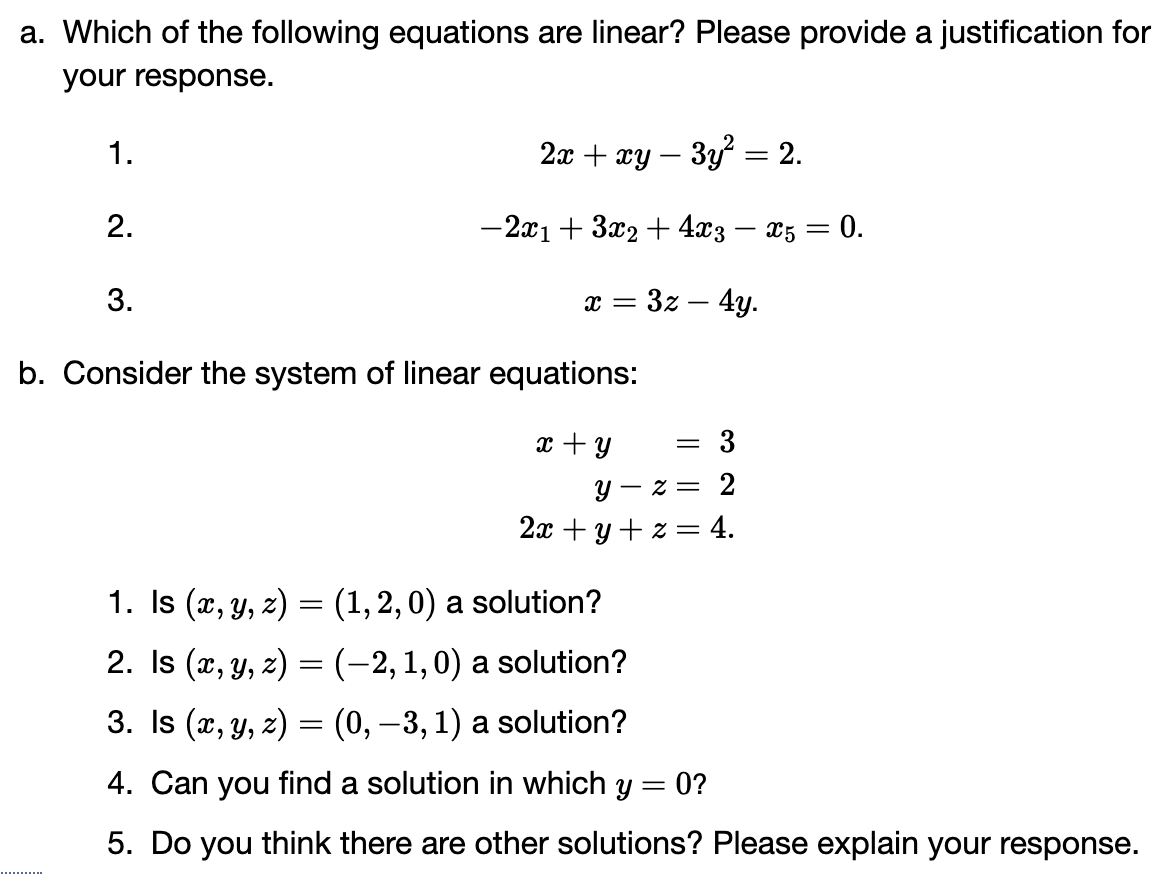
\includegraphics{ge1.pdf}

\begin{center}\rule{0.5\linewidth}{0.5pt}\end{center}

\[\begin{align*}
x + y &= 2000 \\
25x + 50y &= 70000
\end{align*}\]

\begin{tcolorbox}[enhanced jigsaw, coltitle=black, breakable, bottomrule=.15mm, opacitybacktitle=0.6, left=2mm, opacityback=0, rightrule=.15mm, title=\textcolor{quarto-callout-important-color}{\faExclamation}\hspace{0.5em}{Activity}, leftrule=.75mm, toptitle=1mm, colframe=quarto-callout-important-color-frame, toprule=.15mm, colbacktitle=quarto-callout-important-color!10!white, bottomtitle=1mm, titlerule=0mm, arc=.35mm, colback=white]

Using whatever means you can think of, determine if this \(2 \times 2\)
system has a solution. If it doesn't have a solution, be ready to
explain why. If it does have a solution, figure out \emph{how many} it
has, and what it is/they are.

\end{tcolorbox}

\begin{center}\rule{0.5\linewidth}{0.5pt}\end{center}

\hypertarget{there-are-basically-three-ways-to-find-solutions-to-a-system}{%
\subsection{There are basically three ways to find solutions to a
system}\label{there-are-basically-three-ways-to-find-solutions-to-a-system}}

You can \textbf{graph} the equations and see if their graphs intersect.
This works OK for systems with two variables:

\begin{Shaded}
\begin{Highlighting}[]
\ImportTok{from}\NormalTok{ sympy }\ImportTok{import} \OperatorTok{*}
\NormalTok{x, y }\OperatorTok{=}\NormalTok{ symbols(}\StringTok{\textquotesingle{}x y\textquotesingle{}}\NormalTok{)}
\NormalTok{p1 }\OperatorTok{=}\NormalTok{ plot(}\DecValTok{2000} \OperatorTok{{-}}\NormalTok{ x, (x,}\OperatorTok{{-}}\DecValTok{10}\NormalTok{,}\DecValTok{2000}\NormalTok{), show }\OperatorTok{=} \VariableTok{False}\NormalTok{)}
\NormalTok{p2 }\OperatorTok{=}\NormalTok{ plot((}\DecValTok{70000}\OperatorTok{{-}}\DecValTok{25}\OperatorTok{*}\NormalTok{x)}\OperatorTok{/}\DecValTok{50}\NormalTok{, (x, }\OperatorTok{{-}}\DecValTok{10}\NormalTok{, }\DecValTok{2000}\NormalTok{), show }\OperatorTok{=} \VariableTok{False}\NormalTok{)}
\NormalTok{p1.append(p2[}\DecValTok{0}\NormalTok{])}
\NormalTok{p1}
\NormalTok{p1.show()}
\end{Highlighting}
\end{Shaded}

\begin{figure}[H]

{\centering 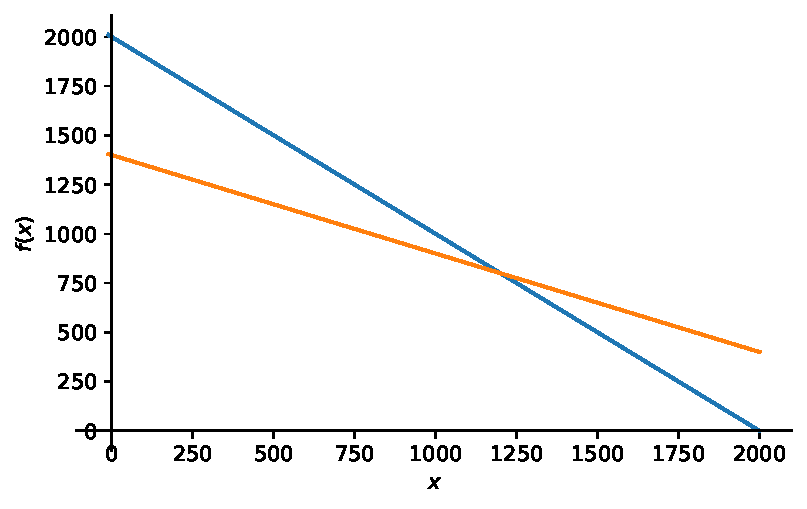
\includegraphics{302-linearsystems_files/figure-pdf/cell-2-output-1.pdf}

}

\end{figure}

\begin{center}\rule{0.5\linewidth}{0.5pt}\end{center}

\ldots but for three variables, it gets weird:

\[\begin{align*}
x + y + z &= 3 \\   
y - z &= 2 \\ 
2x + y + z &= 4 
\end{align*}\]

\begin{Shaded}
\begin{Highlighting}[]
\ImportTok{from}\NormalTok{ sympy.plotting }\ImportTok{import}\NormalTok{ plot3d}
\NormalTok{x,y,z }\OperatorTok{=}\NormalTok{ symbols(}\StringTok{\textquotesingle{}x y z\textquotesingle{}}\NormalTok{)}
\NormalTok{p1 }\OperatorTok{=}\NormalTok{ plot3d(}\DecValTok{3} \OperatorTok{{-}}\NormalTok{ x }\OperatorTok{{-}}\NormalTok{ y, (x,}\OperatorTok{{-}}\DecValTok{5}\NormalTok{,}\DecValTok{5}\NormalTok{), (y,}\OperatorTok{{-}}\DecValTok{5}\NormalTok{,}\DecValTok{5}\NormalTok{), show}\OperatorTok{=}\VariableTok{False}\NormalTok{)}
\NormalTok{p2 }\OperatorTok{=}\NormalTok{ plot3d(y }\OperatorTok{{-}} \DecValTok{2}\NormalTok{, (x,}\OperatorTok{{-}}\DecValTok{5}\NormalTok{,}\DecValTok{5}\NormalTok{), (y,}\OperatorTok{{-}}\DecValTok{5}\NormalTok{,}\DecValTok{5}\NormalTok{), show}\OperatorTok{=}\VariableTok{False}\NormalTok{)}
\NormalTok{p3 }\OperatorTok{=}\NormalTok{ plot3d(}\DecValTok{4} \OperatorTok{{-}} \DecValTok{2}\OperatorTok{*}\NormalTok{x }\OperatorTok{{-}}\NormalTok{ y, (x,}\OperatorTok{{-}}\DecValTok{5}\NormalTok{,}\DecValTok{5}\NormalTok{), (y,}\OperatorTok{{-}}\DecValTok{5}\NormalTok{,}\DecValTok{5}\NormalTok{), show}\OperatorTok{=}\VariableTok{False}\NormalTok{)}
\NormalTok{p1.append(p2[}\DecValTok{0}\NormalTok{])}
\NormalTok{p1.append(p3[}\DecValTok{0}\NormalTok{])}
\NormalTok{p1}
\NormalTok{p1.show()}
\end{Highlighting}
\end{Shaded}

\begin{figure}[H]

{\centering 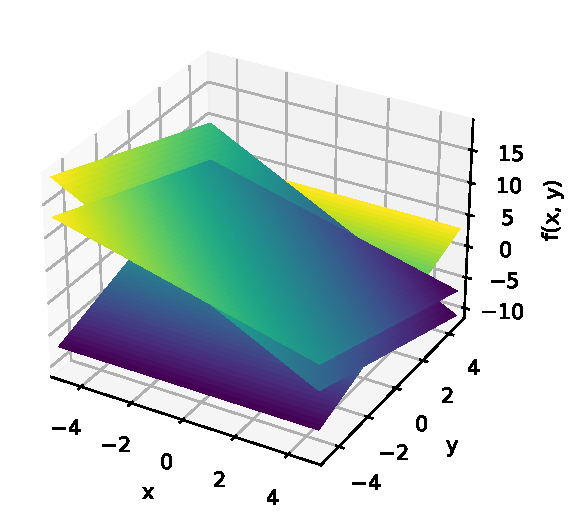
\includegraphics{302-linearsystems_files/figure-pdf/cell-3-output-1.pdf}

}

\end{figure}

\begin{center}\rule{0.5\linewidth}{0.5pt}\end{center}

\hypertarget{but-graphical-intuition-is-very-important-for-us}{%
\subsection{But graphical intuition is very important for
us}\label{but-graphical-intuition-is-very-important-for-us}}

Since solutions to systems are intersections of lines or planes (ir
higher-dimensional versions of these):

\begin{itemize}
\tightlist
\item
  A solution might have solutions (the system is \textbf{consistent}),
  or it might have none (it's \textbf{inconsistent})
\item
  A consistent system can have either \textbf{exactly one} solution, or
  \textbf{infinitely many solutions}, but nothing in between.
\end{itemize}

\href{https://www.desmos.com/calculator/wrajgsvua6}{Check this out}

\begin{center}\rule{0.5\linewidth}{0.5pt}\end{center}

Example of a \emph{consistent} system with \emph{exactly one} solution:
\[\begin{align*}
x + y &= 2 \\
x - y &= 0
\end{align*}\]

Example of a \emph{consistent} system with \emph{infinitely many}
solutions: \[\begin{align*}
x + y &= 2 \\
3x + 3y &= 6
\end{align*}\]

Example of an \emph{inconsistent} system: \[\begin{align*}
x + y &= 2 \\
x + y &= 0
\end{align*}\]

\begin{center}\rule{0.5\linewidth}{0.5pt}\end{center}

Back to solution methods: You could also \textbf{substitute} - Pick an
equation, solve for a variable, plug in to the other equations, and
repeat until you have values. Tedious but doable for 2 or 3 variables.

But this? No thanks: \[\begin{align*}
2x_1 + 3x_2 - x_4 + 3x_5 &= 10 \\
x_2 + x_4 &= 1 \\
-x_1 + 3x_2 + 5x_3 + 2x_4 - 100x_5 &= 0 
\end{align*}\]

\begin{center}\rule{0.5\linewidth}{0.5pt}\end{center}

The best option is \textbf{elimination}. Works by performing a
combination of three \emph{elementary operations}:

\begin{enumerate}
\def\labelenumi{\arabic{enumi}.}
\tightlist
\item
  \emph{Replace} a row, with the sum of itself and a multiple of another
  row.
\item
  \emph{Swap} any two rows.
\item
  \emph{Scale} a row by multiplying both sides by a nonzero constant.
\end{enumerate}

Each operation produces a system that is \textbf{equivalent} to the
original one (it has the same solutions).

At the board: how this works.

\begin{center}\rule{0.5\linewidth}{0.5pt}\end{center}

\(\begin{align*} x + y &= 3 \\ y - z &= 2 \\ 2x + y + z &= 4 \end{align*}\)
\(\Longrightarrow\)
\(\begin{align*} x + z &= 1 \\ y - z &= 2 \\ 0 &= 0 \end{align*}\)

\begin{Shaded}
\begin{Highlighting}[]
\ImportTok{from}\NormalTok{ sympy.plotting }\ImportTok{import}\NormalTok{ plot3d}
\NormalTok{x,y,z }\OperatorTok{=}\NormalTok{ symbols(}\StringTok{\textquotesingle{}x y z\textquotesingle{}}\NormalTok{)}
\NormalTok{p1 }\OperatorTok{=}\NormalTok{ plot3d(}\DecValTok{3} \OperatorTok{{-}}\NormalTok{ x }\OperatorTok{{-}}\NormalTok{ y, (x,}\OperatorTok{{-}}\DecValTok{5}\NormalTok{,}\DecValTok{5}\NormalTok{), (y,}\OperatorTok{{-}}\DecValTok{5}\NormalTok{,}\DecValTok{5}\NormalTok{), show}\OperatorTok{=}\VariableTok{False}\NormalTok{)}
\NormalTok{p2 }\OperatorTok{=}\NormalTok{ plot3d(y }\OperatorTok{{-}} \DecValTok{2}\NormalTok{, (x,}\OperatorTok{{-}}\DecValTok{5}\NormalTok{,}\DecValTok{5}\NormalTok{), (y,}\OperatorTok{{-}}\DecValTok{5}\NormalTok{,}\DecValTok{5}\NormalTok{), show}\OperatorTok{=}\VariableTok{False}\NormalTok{)}
\NormalTok{p1.append(p2[}\DecValTok{0}\NormalTok{])}
\NormalTok{p1}
\NormalTok{p1.show()}
\end{Highlighting}
\end{Shaded}

\begin{figure}[H]

{\centering 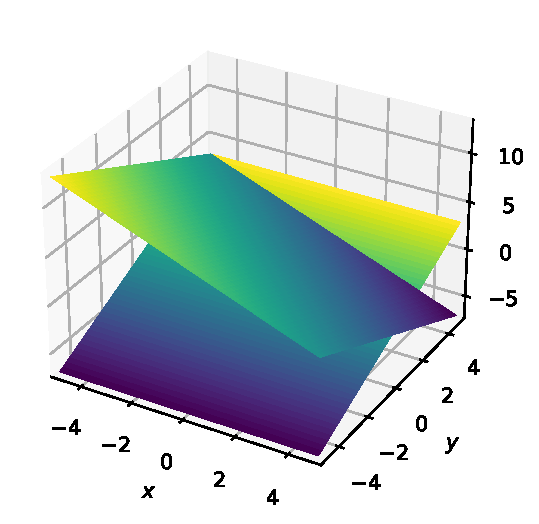
\includegraphics{302-linearsystems_files/figure-pdf/cell-4-output-1.pdf}

}

\end{figure}

\begin{center}\rule{0.5\linewidth}{0.5pt}\end{center}

\begin{tcolorbox}[enhanced jigsaw, coltitle=black, breakable, bottomrule=.15mm, opacitybacktitle=0.6, left=2mm, opacityback=0, rightrule=.15mm, title=\textcolor{quarto-callout-important-color}{\faExclamation}\hspace{0.5em}{KEY INSIGHT}, leftrule=.75mm, toptitle=1mm, colframe=quarto-callout-important-color-frame, toprule=.15mm, colbacktitle=quarto-callout-important-color!10!white, bottomtitle=1mm, titlerule=0mm, arc=.35mm, colback=white]

The variables in the elimination process don't matter that much. They
are just there as placeholders for the coefficients. So forget them and
put the coefficients and right-hand sides into an array called the
\textbf{augmented matrix} for the system.

\end{tcolorbox}

\[\begin{align*}
x + y + z &= 3 \\   
y - z &= 2 \\ 
2x + y + z &= 4 
\end{align*}\]

\[\begin{bmatrix}
1 & 1 & 1 & 3 \\ 
0 & 1 & -1 & 2 \\ 
2 & 1 & 1 & 4
\end{bmatrix}\] Now you can do elimination just with the matrix. (Board)

\begin{center}\rule{0.5\linewidth}{0.5pt}\end{center}

\[\begin{equation*}
\begin{alignedat}{4}
x &  {}+{}  & 2y &  &  &  {}={}  & 4 \\
2x &  {}+{}  & y &  {}-{}  & 3z &  {}={}  & 11 \\
-3x &  {}-{}  & 2y &  {}+{}  & z &  {}={}  & -10 \\
\end{alignedat}
\end{equation*}\]

\begin{tcolorbox}[enhanced jigsaw, coltitle=black, breakable, bottomrule=.15mm, opacitybacktitle=0.6, left=2mm, opacityback=0, rightrule=.15mm, title=\textcolor{quarto-callout-important-color}{\faExclamation}\hspace{0.5em}{Activity}, leftrule=.75mm, toptitle=1mm, colframe=quarto-callout-important-color-frame, toprule=.15mm, colbacktitle=quarto-callout-important-color!10!white, bottomtitle=1mm, titlerule=0mm, arc=.35mm, colback=white]

Convert this system into an augmented matrix. Then use a sequence of the
three elementary operations to try to find a solution (there may not be
one).

\end{tcolorbox}

\begin{center}\rule{0.5\linewidth}{0.5pt}\end{center}

\begin{Shaded}
\begin{Highlighting}[]
\ImportTok{from}\NormalTok{ sympy }\ImportTok{import} \OperatorTok{*} 
\NormalTok{init\_printing()}
\NormalTok{M }\OperatorTok{=}\NormalTok{ Matrix(}\DecValTok{3}\NormalTok{,}\DecValTok{4}\NormalTok{, [}\DecValTok{1}\NormalTok{,}\DecValTok{2}\NormalTok{,}\DecValTok{0}\NormalTok{,}\DecValTok{4}\NormalTok{,}\DecValTok{2}\NormalTok{,}\DecValTok{1}\NormalTok{,}\OperatorTok{{-}}\DecValTok{3}\NormalTok{,}\DecValTok{11}\NormalTok{, }\OperatorTok{{-}}\DecValTok{3}\NormalTok{, }\OperatorTok{{-}}\DecValTok{2}\NormalTok{, }\DecValTok{1}\NormalTok{, }\OperatorTok{{-}}\DecValTok{10}\NormalTok{])}
\NormalTok{M.rref(pivots }\OperatorTok{=} \VariableTok{False}\NormalTok{)}
\end{Highlighting}
\end{Shaded}

$\displaystyle \left[\begin{matrix}1 & 0 & 0 & 2\\0 & 1 & 0 & 1\\0 & 0 & 1 & -2\end{matrix}\right]$

This matrix is in \textbf{reduced row echelon form (RREF)}:

\begin{itemize}
\tightlist
\item
  If there are any rows that are all zero, they are at the bottom.
\item
  The first nonzero entry in a given row is \(1\), and it's in a column
  that's to the right of the first nonzero entry in any row above it.
\item
  Every other entry in a column with a leading \(1\) is \(0\).
\end{itemize}

\begin{center}\rule{0.5\linewidth}{0.5pt}\end{center}

Consistent with one solution: \[\begin{bmatrix}
1 & 0 & 2 \\
0 & 1 & -5 
\end{bmatrix}\]

Consistent with infinitely many solutions: \[\begin{bmatrix}
1 & 0 & 2 & 1 \\
0 & 1 & -1 & -5  
\end{bmatrix}\]

Inconsistent: \[\begin{bmatrix}
1 & 0 & 2 \\
0 & 0 & -5 
\end{bmatrix}\]

\begin{center}\rule{0.5\linewidth}{0.5pt}\end{center}

\[\begin{bmatrix}
1 & 0 & 2 & 1 \\
0 & 1 & -1 & -5  
\end{bmatrix}\]

Is shorthand for the system \[\begin{align*}
x_1 + 2x_3 &= 1 \\  
x_2 - x_3 &= -5
\end{align*}\] To find a solution: Pick anything for \(x_3\). Then
\(x_1 = 1 - 2x_3\) and \(x_2 = x_3 - 5\).

\begin{itemize}
\tightlist
\item
  \(x_3\) is a \textbf{free variable}
\item
  \(x_1\) and \(x_2\) are \textbf{pivots} or sometimes ``determined'' or
  ``dependent'' variables
\end{itemize}

\begin{center}\rule{0.5\linewidth}{0.5pt}\end{center}

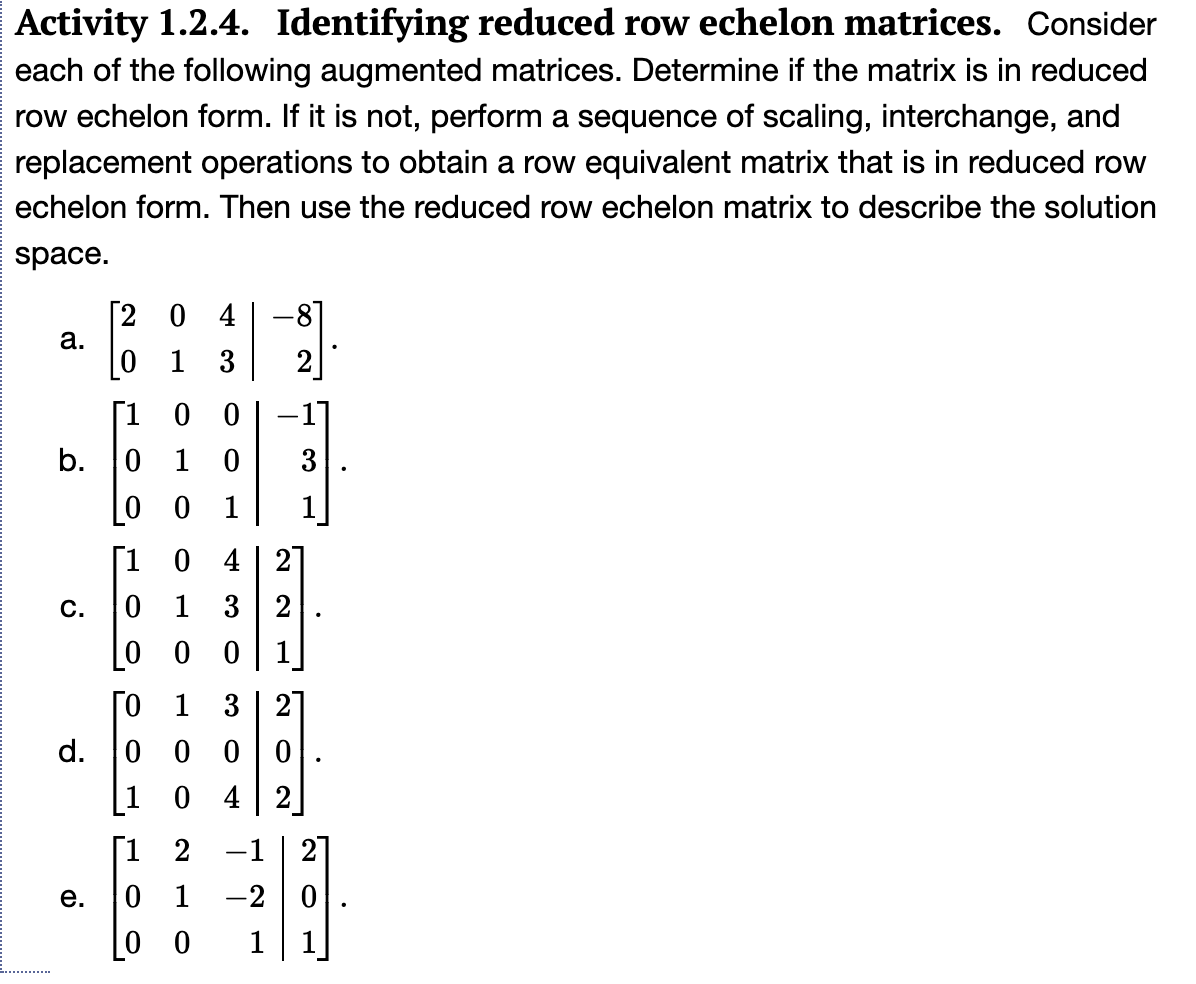
\includegraphics{ge2.pdf}

\begin{center}\rule{0.5\linewidth}{0.5pt}\end{center}

\begin{figure}[H]

{\centering 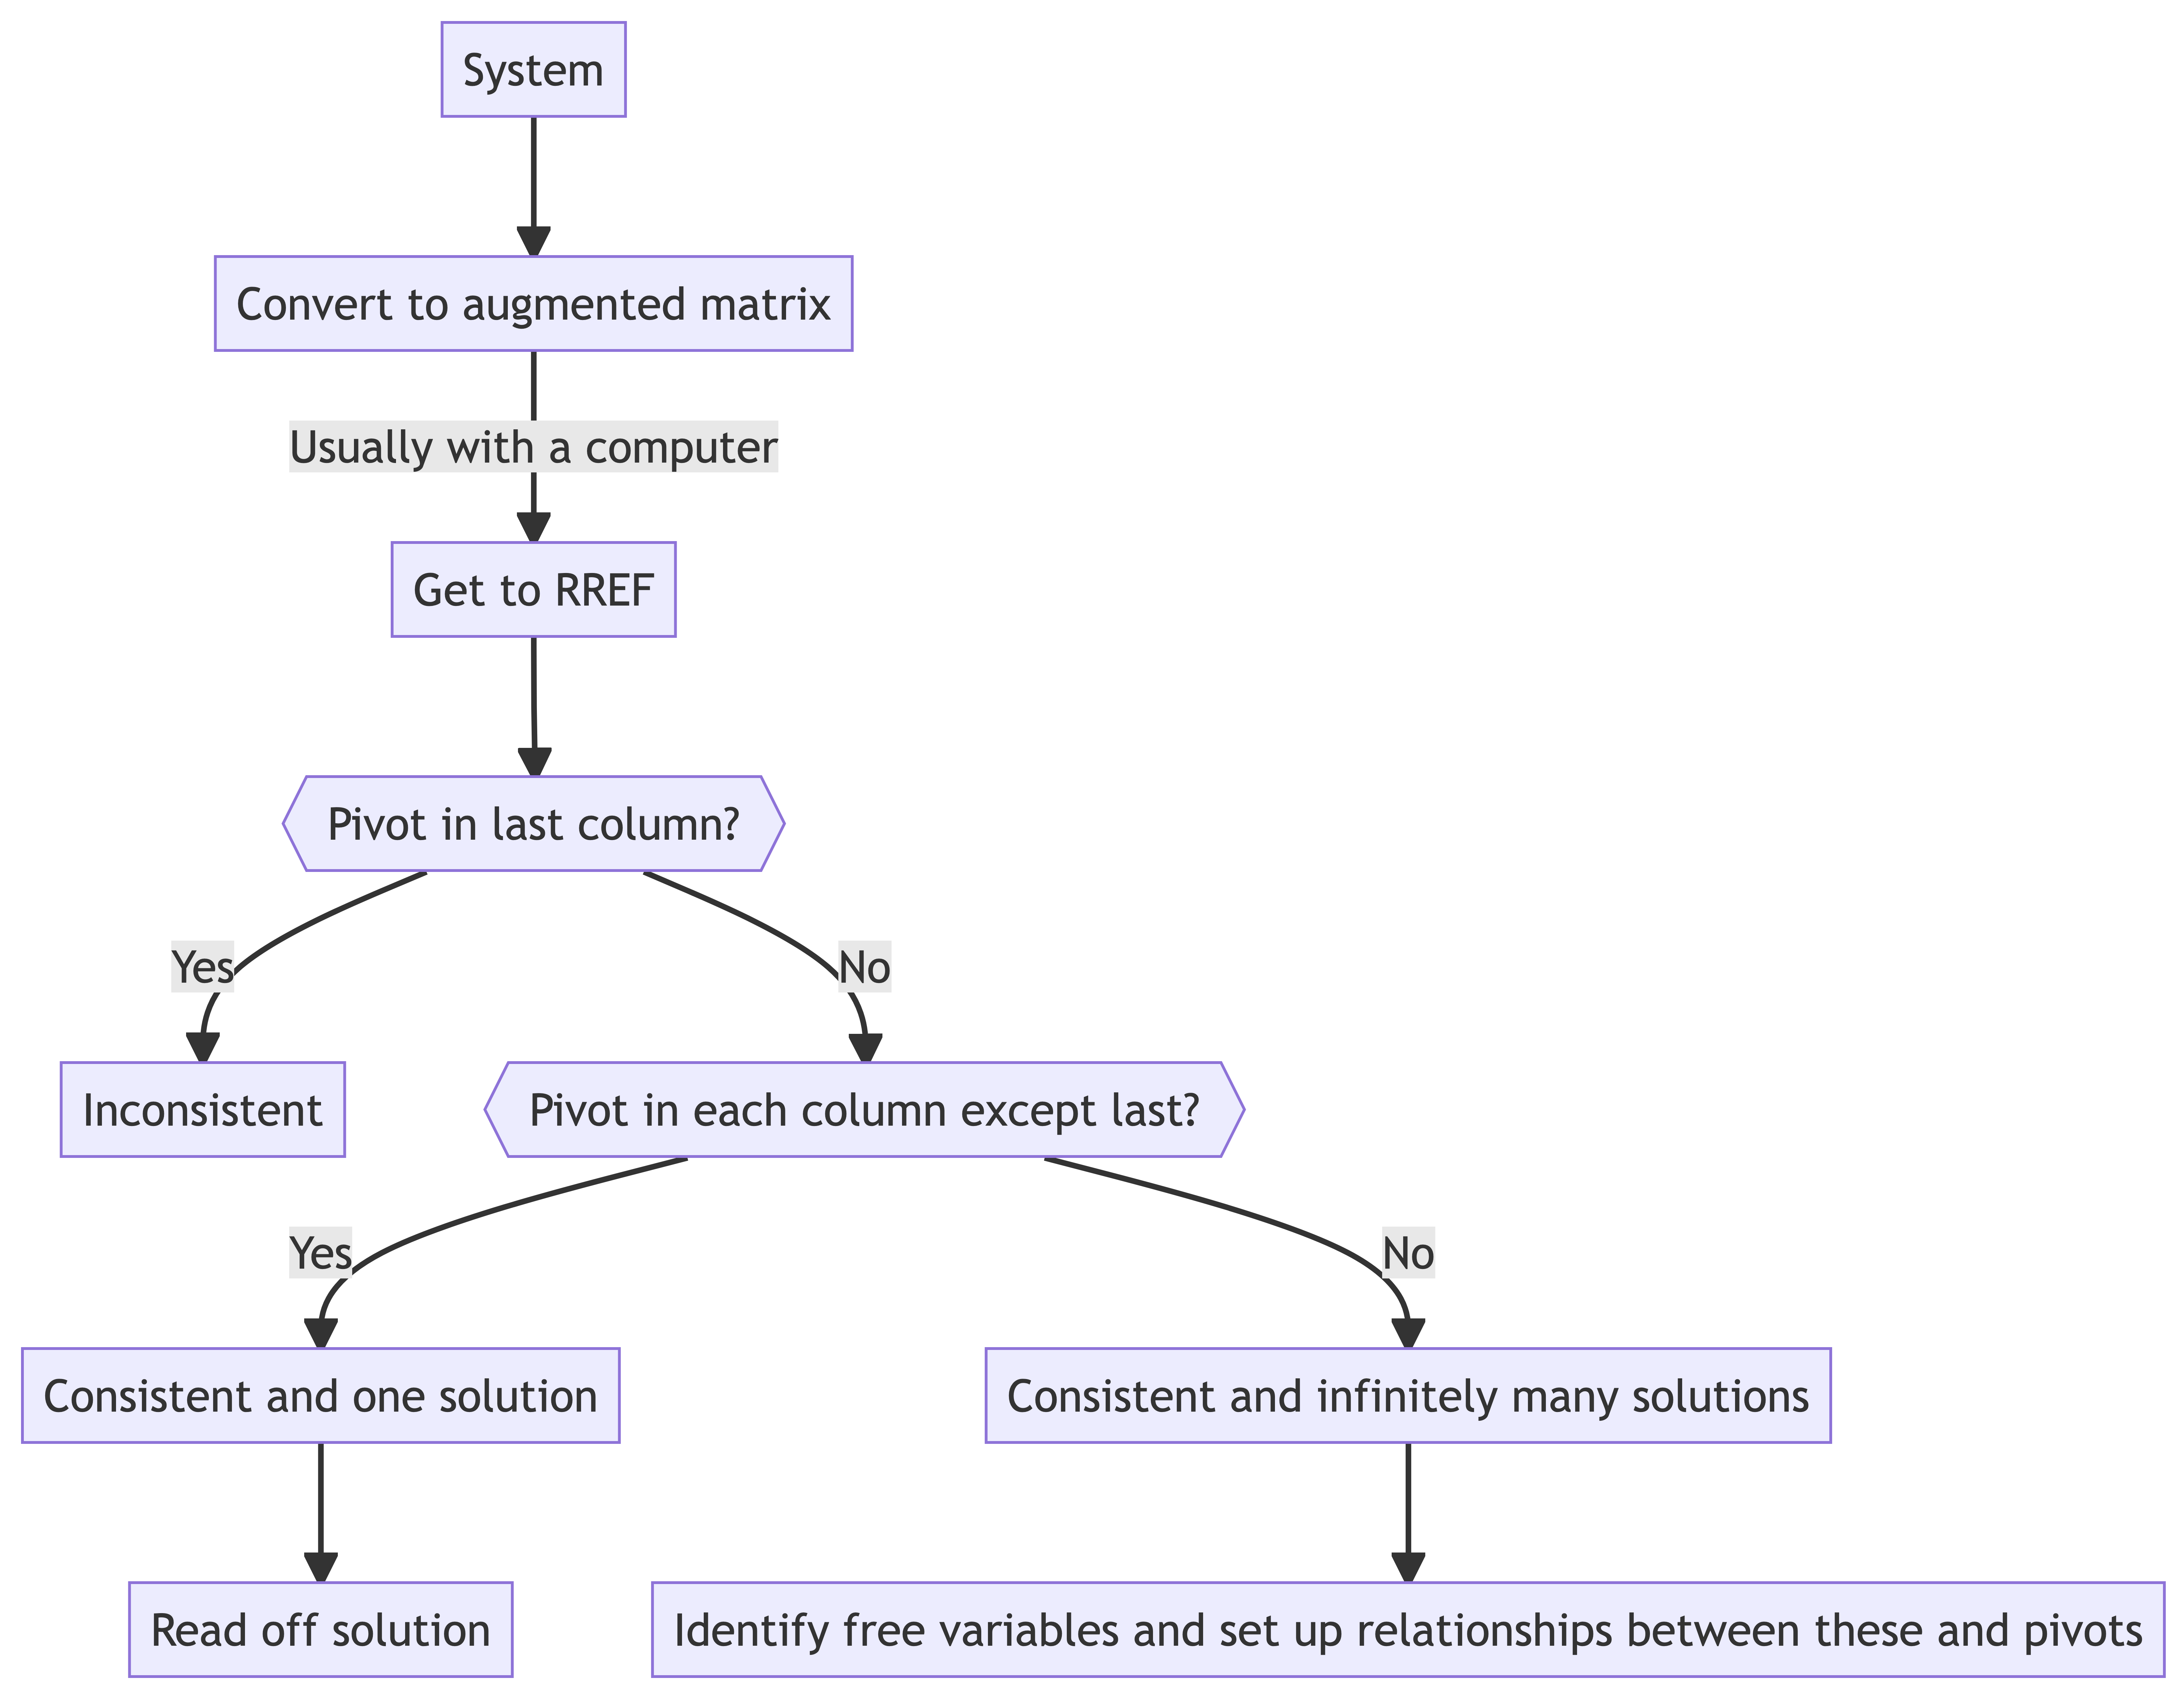
\includegraphics[width=8.12in,height=6.31in]{302-linearsystems_files/figure-latex/mermaid-figure-1.png}

}

\end{figure}

\begin{center}\rule{0.5\linewidth}{0.5pt}\end{center}

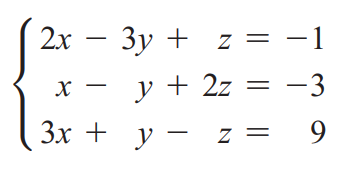
\includegraphics{system.png}

\begin{itemize}
\tightlist
\item
  Convert this to an augmented matrix
\item
  Get the matrix into RREF
\item
  Determine if the system is consistent or inconsistent
\item
  If consistent, decide whether there is one solution or infinitelky
  many
\item
  If just one, determine what it is
\item
  If infinitely many, identify the free variable(s) and a relationship
  between the pivot variables and the free variables
\end{itemize}

\begin{center}\rule{0.5\linewidth}{0.5pt}\end{center}

\hypertarget{more-facts-about-rref}{%
\subsection{More facts about RREF}\label{more-facts-about-rref}}

\begin{itemize}
\tightlist
\item
  The process of putting a matrix into RREF is called
  \textbf{Gauss-Jordan elimination} and it's kind of a big deal
\item
  \emph{Skill LA.1: I can solve a system of linear equations by
  converting it into an augmented matrix and putting into reduced row
  echelon form}. Coming next Thursday on Skill Quiz 1 and in Practice
  Set 1.
\item
  \textbf{But this is the only place you will be asked to do elimination
  by hand!} In all other situations you will use a computer.
\item
  So don't stress over doing RREF by hand, just practice until you can
  do it on simple systems without a bunch of mistakes. \(\rightarrow\)
  \textbf{Optional RREF Practice set on WeBWorK}
\end{itemize}

\begin{center}\rule{0.5\linewidth}{0.5pt}\end{center}

\hypertarget{next}{%
\subsection{Next}\label{next}}

\begin{itemize}
\tightlist
\item
  Remainder of today: Choose your adventure. Get 1-1 help; work on
  Practice Set 1; work on Startup tasks; work on RREF practice; (Section
  04 only) Please put tables back in rows
\item
  Sunday: Complete Practice Set 1 by 11:59pm ET
\item
  Tuesday:

  \begin{itemize}
  \tightlist
  \item
    Complete Class Prep for Jan 17 (Blackboard \textgreater{} Class
    Prep) by 11:59pm ET \textbf{Monday}
  \item
    Focus for Tuesday: Linear combinations of vectors (and what this has
    to do with solutions to systems)
  \end{itemize}
\end{itemize}



\end{document}
